\chapter{Data Preprocessing}
\label{ch:data_preprocessing}

\section{Dataset}
\label{sec:dataset}

The dataset contains a file named isles24\_multimodal\_5fold\_NIHSSstratified.json which contains some useful information about the Dataset. It is divided into five folds as shown by the "fold" field for each case. The split is stratified by NIHSS scores, meaning that each fold has a balanced distribution of stroke severity, which ensures that cross-validation results are robust and representative of the entire cohort.

\subsection{Dataset Structure}
\label{subsec:dataset_structure}

The dataset is organized into three main subdirectories: "derivatives", "phenotype", and "raw\_data". 
\begin{itemize}
    \item "raw\_data" contains the original data from the ISLES24 challenge.
    \item "phenotype" contains clinical and demographic information about the patients.
    \item "derivatives" contains the processed data for each patient.
\end{itemize}

The tree subdirectories have a similar structure to the following example of derivatives for patient SUB-STROKE0001:
Since the folder structure is somewhat complex, we use the \texttt{tree path /F} command to visualize the structure of one patient's data (stored in SUB-STROKE0001). Each patient in the dataset has a similar directory structure:
\begin{verbatim}
D:\TUM_CLINICAL_PROJECT\ISLES24_COMBINED\DERIVATIVES\SUB-STROKE0001
+---ses-01
|   |   sub-stroke0001_ses-01_space-ncct_cta.nii.gz
|   |   sub-stroke0001_ses-01_space-ncct_ctp.nii.gz
|   |
|   \---perfusion-maps
|           sub-stroke0001_ses-01_space-ncct_cbf.nii.gz
|           sub-stroke0001_ses-01_space-ncct_cbv.nii.gz
|           sub-stroke0001_ses-01_space-ncct_mtt.nii.gz
|           sub-stroke0001_ses-01_space-ncct_tmax.nii.gz
|
\---ses-02
            sub-stroke0001_ses-02_lesion-msk.nii.gz
\end{verbatim}

As shown above, the patient data is organized into two sessions:
\begin{itemize}
    \item \textbf{ses-01}: Contains the CT angiography (CTA) and CT perfusion (CTP) scans, acquired in the acute phase, along with derived perfusion maps (cerebral blood flow, cerebral blood volume, mean transit time, and time-to-maximum).
    \item \textbf{ses-02}: Contains the lesion mask derived from follow-up MRI, which serves as the ground truth for our prediction task.
\end{itemize}

This structure follows the BIDS (Brain Imaging Data Structure) format, which is a standardized way of organizing neuroimaging data. The naming convention includes subject ID, session, image space, and modality, making it easier to identify and process the files programmatically.

% Content for the data preprocessing chapter will be added here 
\section{Registration}
\label{sec:registration}
Even though the data has already been registirated we double check this by writing a short script. 
We compare the affine matrix of the first images of the CT, perfusion and lesion. 
We get the following results:

\begin{lstlisting}[breaklines=true, basicstyle=\ttfamily\small]
Filename: sub-stroke0001_ses-01_space-ncct_cta.nii.gz
(-120.0, 254.75277709960938, -58.179813385009766)
(0.46875, 0.46875, 2.0)
(1.0, 0.0, 0.0, 0.0, -0.9659258450112692, -0.25881896370865276, 0.0, 0.25881897523030545, -0.9659258480984858)
(512, 595, 75)
Filename: sub-stroke0001_ses-01_space-ncct_ctp.nii.gz
(-120.0, 216.44757080078125, -201.1368408203125)
(0.46875, 0.46875, 2.0)
(1.0, 0.0, 0.0, 0.0, 1.0, 0.0, 0.0, 0.0, 1.0)
(512, 595, 75)
Filename: sub-stroke0001_ses-02_lesion-msk.nii.gz
(-120.0, 254.75277709960938, -58.17981719970703)
(0.46875, 0.46875, 2.0)
(1.0, 0.0, 0.0, 0.0, -0.9659258410376269, -0.2588189915146001, 0.0, 0.25881899006014436, -0.9659258406479068)
(512, 595, 75)
Filename: sub-stroke0001_ses-01_space-ncct_cbf.nii.gz
(-120.0, 254.75277709960938, -58.17981719970703)
(0.46875, 0.46875, 2.0)
(1.0, 0.0, 0.0, 0.0, -0.9659258410376269, -0.2588189915146001, 0.0, 0.25881899006014436, -0.9659258406479068)
(512, 595, 75)
Filename: sub-stroke0001_ses-01_space-ncct_cbv.nii.gz
(-120.0, 254.75277709960938, -58.17981719970703)
(0.46875, 0.46875, 2.0)
(1.0, 0.0, 0.0, 0.0, -0.9659258410376269, -0.2588189915146001, 0.0, 0.25881899006014436, -0.9659258406479068)
(512, 595, 75)
Filename: sub-stroke0001_ses-01_space-ncct_mtt.nii.gz
(-120.0, 254.75277709960938, -58.17981719970703)
(0.46875, 0.46875, 2.0)
(512, 595, 75)
Filename: sub-stroke0001_ses-01_space-ncct_tmax.nii.gz
(-120.0, 254.75277709960938, -58.17981719970703)
(0.46875, 0.46875, 2.0)
(1.0, 0.0, 0.0, 0.0, -0.9659258410376269, -0.2588189915146001, 0.0, 0.25881899006014436, -0.9659258406479068)
(512, 595, 75)
\end{lstlisting}

We see that the affine matrix is the same for all images except for the lesion mask. (This is fine as the lesion mask is not registered)

\section{Normalization}
\label{sec:normalization}

Medical images from different sources can have significant variations in intensity values due to differences in imaging protocols, scanner hardware, and acquisition parameters. To address this variability and improve the performance of machine learning models, we apply Z-score normalization to our dataset.

\subsection{Z-Score Normalization}
\label{subsec:z_score_normalization}

Z-score normalization (also known as standardization) transforms the intensity values of an image to have a mean of 0 and a standard deviation of 1. For each voxel value $x$ in the dataset, the normalization formula is:

\begin{equation}
z = \frac{x - \mu}{\sigma}
\end{equation}

where $\mu$ is the mean intensity value of the entire volume and $\sigma$ is the standard deviation.

This normalization technique offers several advantages for medical image analysis:
\begin{itemize}
    \item It centers the data distribution around zero, making different scans more comparable
    \item It helps deep learning models converge faster during training
    \item It reduces the influence of variations in scanner settings and image acquisition parameters
\end{itemize}

\subsection{Normalization Script}
\label{subsec:normalization_implementation}

To make sure that we work with normalized data, I developed a Python script that iterates over all the NIfTI files in our dataset and applies Z-score normalization to them. In addition, the script visualizes the original and normalized images side by side and the difference map.


Figure \ref{fig:normalization_example} demonstrates the effects of Z-score normalization on a CT scan slice. This visualization highlights several important observations about the normalization process:

\begin{figure}[htbp]
    \centering
    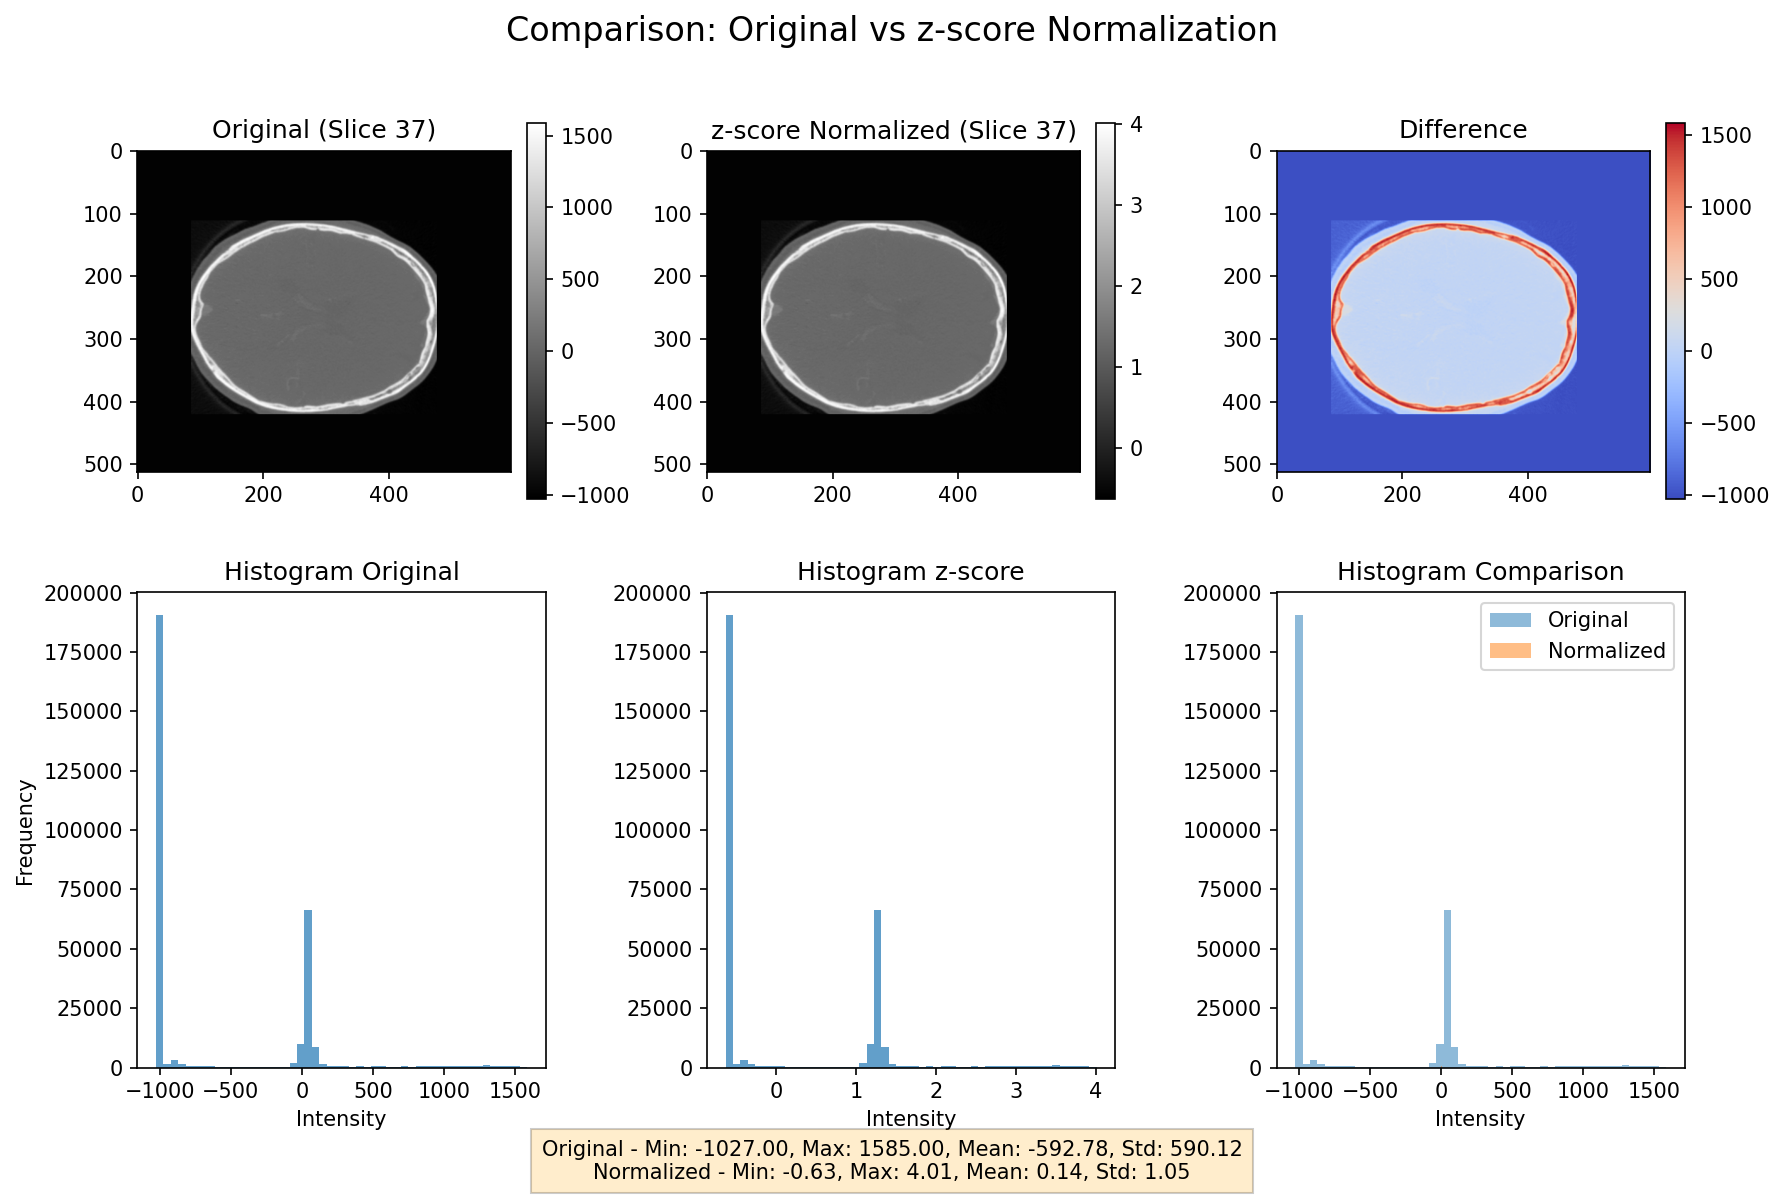
\includegraphics[width=\textwidth]{figures/normalization_example.png}
    \caption{Example of Z-score normalization applied to a CT image (slice 37). Top row: Original image (left), normalized image (center), and difference map (right). Bottom row: Corresponding histograms showing intensity distributions before and after normalization. Note the significant change in intensity range and scale after normalization.}
    \label{fig:normalization_example}
\end{figure}

As clearly illustrated in Figure \ref{fig:normalization_example}, Z-score normalization has several observable effects:

\begin{itemize}
    \item \textbf{Range transformation:} The original image has intensity values ranging from approximately -1027 to 1585, while the normalized image values are scaled to approximately -0.63 to 4.01. This demonstrates how the normalization process compresses the wide range of CT Hounsfield units into a standardized range centered around zero.
    
    \item \textbf{Statistical properties:} The mean value of the original image is -592.78 with a standard deviation of 590.12. After normalization, the mean is much closer to zero (0.14) with a standard deviation close to one (1.05), which closely aligns with the goal of Z-score normalization.
    
    \item \textbf{Contrast preservation:} Despite the intensity value transformation, the normalized image preserves the important structural features and contrast relationships of the original image.
   
    \item \textbf{Difference map:} The difference image (top right) highlights where the most significant changes occurred. The skull region shows the most pronounced transformation (in red), which is expected given that bone has the highest Hounsfield unit values in CT scans.
    
    \item \textbf{Histogram redistribution:} The bottom row histograms reveal how normalization transforms the intensity distribution. While maintaining the general bimodal shape (representing primarily air/background and soft tissue/bone), the distribution is rescaled to center around zero, making it more suitable for deep learning algorithms.
\end{itemize}

This standardization process ensures that intensity values across different scans become comparable, which is particularly important when training machine learning models on datasets acquired from different scanners or institutions.

\textbf{Note:} I created this script to work with my local directory structure. If you wish to use this script, please modify the file paths to match your directory structure.